% Ubah judul dan label berikut sesuai dengan yang diinginkan.
\section{Metodologi}
\label{sec:metodologi}

% Ubah paragraf-paragraf pada bagian ini sesuai dengan yang diinginkan.

Penelitian ini dilaksanakan sesuai dengan desain sistem berikut ini beserta implementasinya. Desain sistem merupakan konsep dari pembuatan dan perencangan infrastruktur dan kemudian diwujudkan dalam bentuk blok-blok alur yang harus dikerjakan.

Pada penelitian ini akan dibuat suatu alat yang terintegrasi dengan teknologi visi komputer untuk mengontrol gerak kursi roda. Secara umum penelitian kali ini akan menggunakan desain sistem sesuai dengan Gambar \ref{fig:Metodologi Penelitian}.

% Gambar 3.1
\begin{figure} [ht] \centering
    % Nama dari file gambar yang diinputkan
    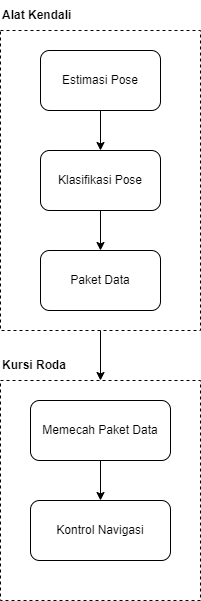
\includegraphics[scale=0.68]{gambar/blokDiagram.png}
    % Keterangan gambar yang diinputkan
    \caption{Blok Diagram Penelitian}
    % Label referensi dari gambar yang diinputkan
    \label{fig:Metodologi Penelitian}
\end{figure}

\subsection{Estimasi Pose}
Deteksi pose merupakan suatu proses yang melibatkan penggunaan bahasa pemrograman Python bersama dengan \emph{library} OpenCV dan \emph{framework} Mediapipe. Dalam konteks ini, Mediapipe berperan penting dalam mendapatkan informasi titik-titik \emph{landmark} yang signifikan pada objek yang diidentifikasi. \emph{Landmark} ini kemudian menjadi dasar untuk membentuk suatu representasi visual yang memvisualisasikan pose tersebut. Proses selanjutnya melibatkan penghubungan titik-titik \emph{landmark} yang telah ditentukan, di mana garis-garis dibuat untuk menggambarkan relasi spasial antar titik-titik tersebut. Dengan demikian, prosedur ini tidak hanya mengandalkan Mediapipe sebagai \emph{framework} utama, tetapi juga memanfaatkan OpenCV sebagai alat bantu untuk analisis citra dan manipulasi visual yang diperlukan dalam deteksi pose.

Pada penelitian kali ini akan memanfaatkan teknologi \emph{hand pose} dari Mediapipe untuk mengontrol gerak kursi roda. Terdapat beberapa titik \emph{keypoints} yang akan digunakan pada estimasi pose ini. Titik \emph{keypoints} yang akan digunakan pada estimasi  pose ini dapat dilihat pada Tabel \ref{tbl:titik keypoints}.

\begin{table}[h]
  \caption{Tabel Titik Keypoints Yang Relevan Pada Estimasi Pose\cite{Developer_2023}}
  \label{tbl:titik keypoints}
  \centering
  \begin{tabular}{|c|c|}
    \hline
    Nomor Keypoint & Nama Keypoint      \\ \hline
    0              & Pergelangan Tangan \\ \hline
    1              & CMC Ibu Jari       \\ \hline
    2              & MPM Ibu Jari       \\ \hline
    3              & IP Ibu Jari        \\ \hline
    4              & TIP Ibu Jari       \\ \hline
    5              & MCP Telunjuk       \\ \hline
    6              & PIP Telunjuk       \\ \hline
    7              & DIP Telunjuk       \\ \hline
    8              & TIP Telunjuk       \\ \hline
    9              & MCP Jari Tengah    \\ \hline
    10             & PIP Jari Tengah    \\ \hline
    11             & DIP Jari Tengah    \\ \hline
    12             & TIP Jari Tengah    \\ \hline
    13             & MCP Jari Manis     \\ \hline
    14             & PIP Jari Manis     \\ \hline
    15             & DIP Jari Manis     \\ \hline
    16             & TIP Jari Manis     \\ \hline
    17             & MCP Kelingking     \\ \hline
    18             & PIP Kelingking     \\ \hline
    19             & DIP Kelingking     \\ \hline
    20             & TIP Kelingking     \\ \hline
  \end{tabular}
\end{table}

Setiap titik \emph{landmark} yang terdapat pada peraga akan diwarnai dengan warna yang unik untuk membedakan setiap jarinya. Secara spesifik, warna yang diberikan pada setiap titik \emph{landmark} mencerminkan asosiasi dengan jari tertentu, sehingga menciptakan representasi visual yang lebih terperinci dan informatif. Untuk memberikan gambaran yang lebih konkret maka berikut ini contoh citra yang telah diestimasi pose yang dapat dilihat pada Gambar \ref{fig:contoh citra yang telah diestimasi pose}.

\begin{figure} [ht] \centering
  % Nama dari file gambar yang diinputkan
  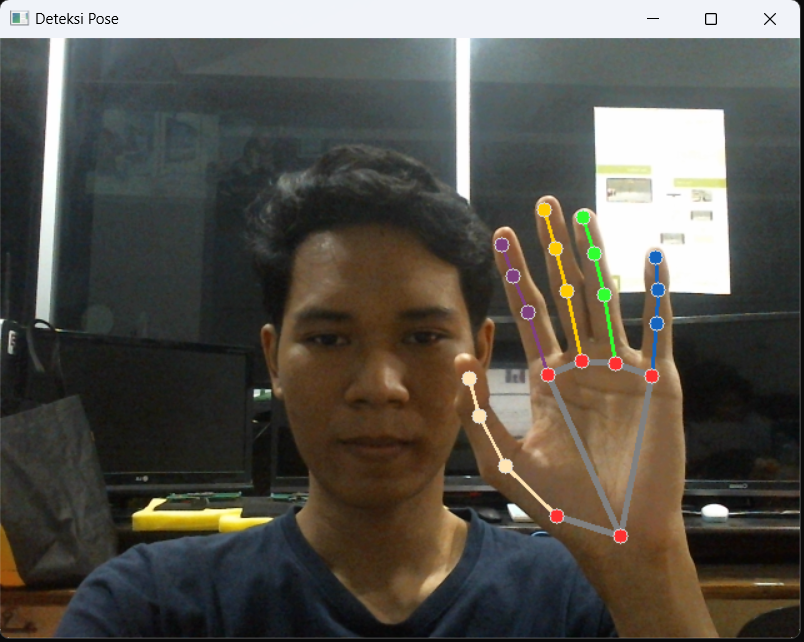
\includegraphics[scale=0.5]{gambar/bab3/EstimasiPose.png}
  % Keterangan gambar yang diinputkan
  \caption{Contoh citra yang telah diestimasi pose}
  % Label referensi dari gambar yang diinputkan
  \label{fig:contoh citra yang telah diestimasi pose}
\end{figure}

\newpage

\subsection{Klasifikasi Pose}
Setelah proses estimasi pose tangan selesai, maka langkah selanjutnya ada mengelompokkan citra-citra hasil estimasi menjadi suatu dataset. Dataset ini akan memiliki 5 kelas berbeda yang masing-masing merepresentasikan perintah untuk maju, mundur, bergerak ke kanan, bergerak ke kiri, dan berhenti. Kelas ini mewakili perintah dasar untuk menggerakkan kursi roda. 

Untuk meningkatkan kinerja dan akurasi maka dataset ini kemudian akan melewati proses \emph{training} menggunakan algoritma \emph{Convolutional Neural Network} (CNN). Penggunaan CNN dalam \emph{training} dataset diharapkan dapat menghasilkan model yang mampu mengenali pola dan fitur yang kompleks, sehingga memungkinkan sistem untuk merespon dengan tepat terhadap variasi perintah yang mungkin diberikan oleh peraga. Hasil dari model prediksi yang telah dibuat dapat dilihat pada Gambar \ref{fig:klasifikasi kiri}, Gambar \ref{fig:klasifikasi maju}, Gambar \ref{fig:klasifikasi stop}, Gambar \ref{fig:klasifikasi mundur}, dan Gambar \ref{fig:klasifikasi kanan}.

\begin{figure} [h] \centering
  % Nama dari file gambar yang diinputkan
  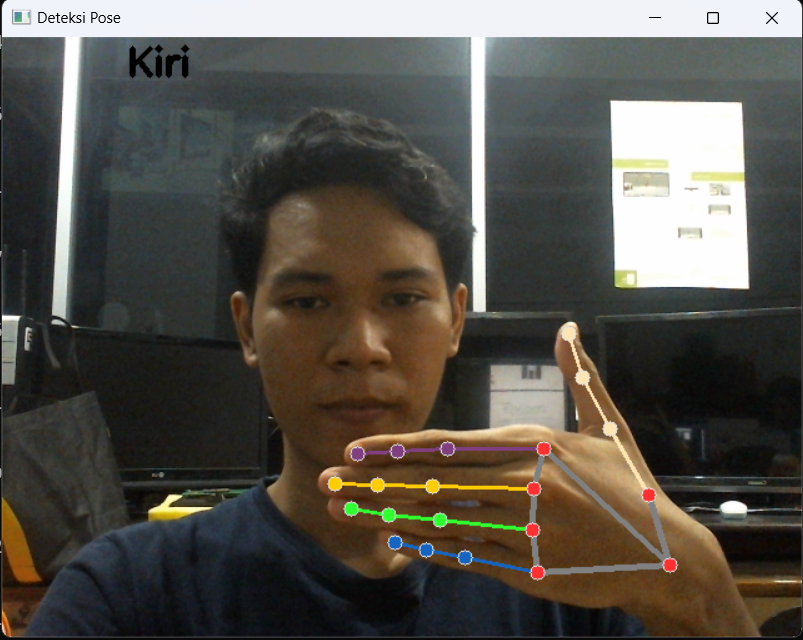
\includegraphics[scale=0.48]{gambar/bab3/Kiri.png}
  % Keterangan gambar yang diinputkan
  \caption{Contoh citra yang mendeteksi kiri}
  % Label referensi dari gambar yang diinputkan
  \label{fig:klasifikasi kiri}
\end{figure}

\newpage

\begin{figure} [h] \centering
  % Nama dari file gambar yang diinputkan
  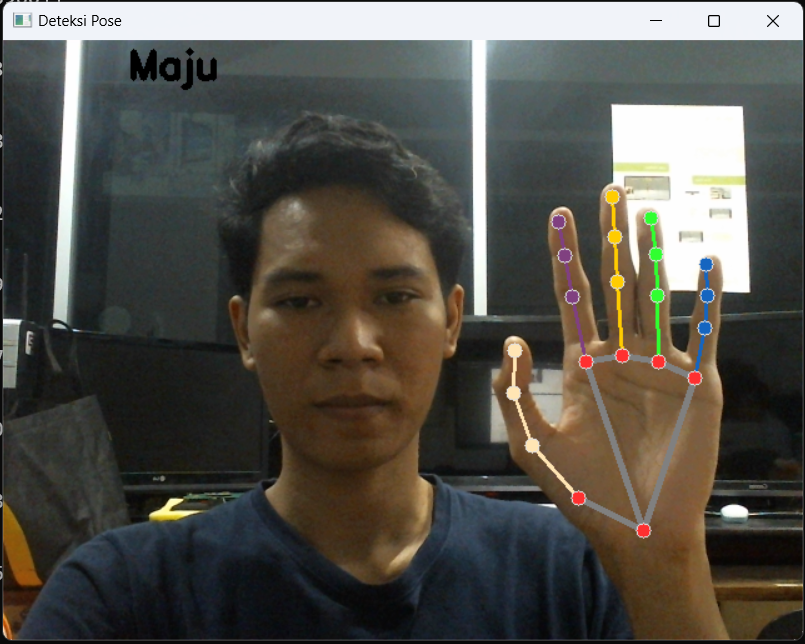
\includegraphics[scale=0.473]{gambar/bab3/Maju.png}
  % Keterangan gambar yang diinputkan
  \caption{Contoh citra yang mendeteksi maju}
  % Label referensi dari gambar yang diinputkan
  \label{fig:klasifikasi maju}
\end{figure}

\begin{figure} [h] \centering
  % Nama dari file gambar yang diinputkan
  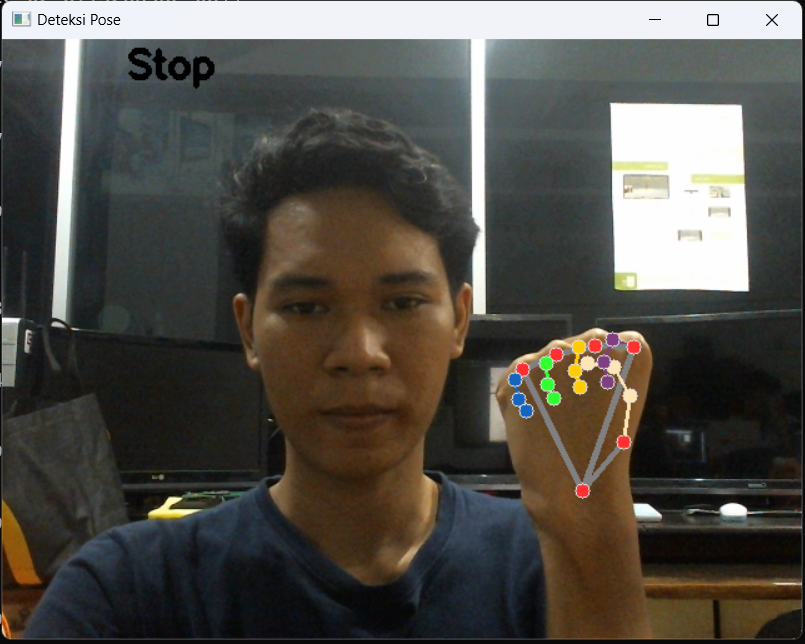
\includegraphics[scale=0.473]{gambar/bab3/Stop.png}
  % Keterangan gambar yang diinputkan
  \caption{Contoh citra yang mendeteksi stop}
  % Label referensi dari gambar yang diinputkan
  \label{fig:klasifikasi stop}
\end{figure}

\begin{figure} [!ht] \centering
  % Nama dari file gambar yang diinputkan
  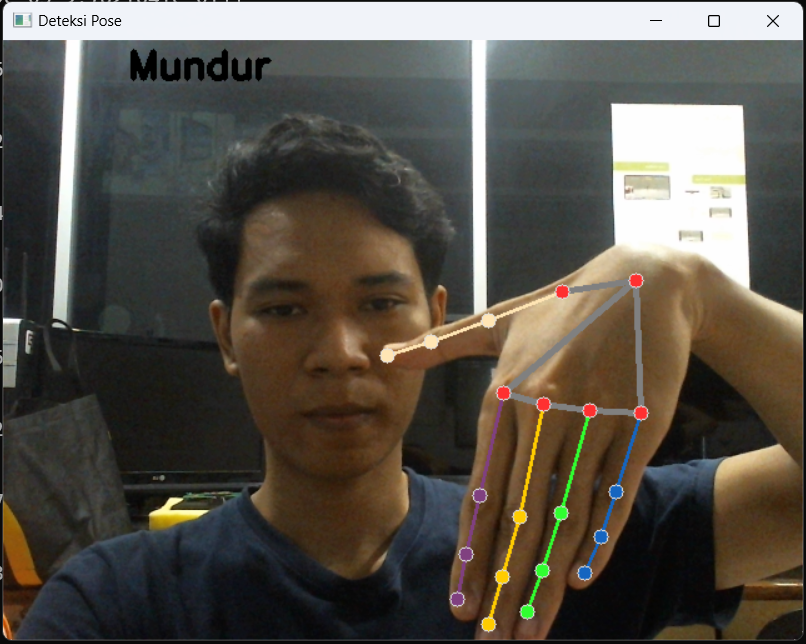
\includegraphics[scale=0.473]{gambar/bab3/Mundur.png}
  % Keterangan gambar yang diinputkan
  \caption{Contoh citra yang mendeteksi mundur}
  % Label referensi dari gambar yang diinputkan
  \label{fig:klasifikasi mundur}
\end{figure}

\begin{figure} [h] \centering
  % Nama dari file gambar yang diinputkan
  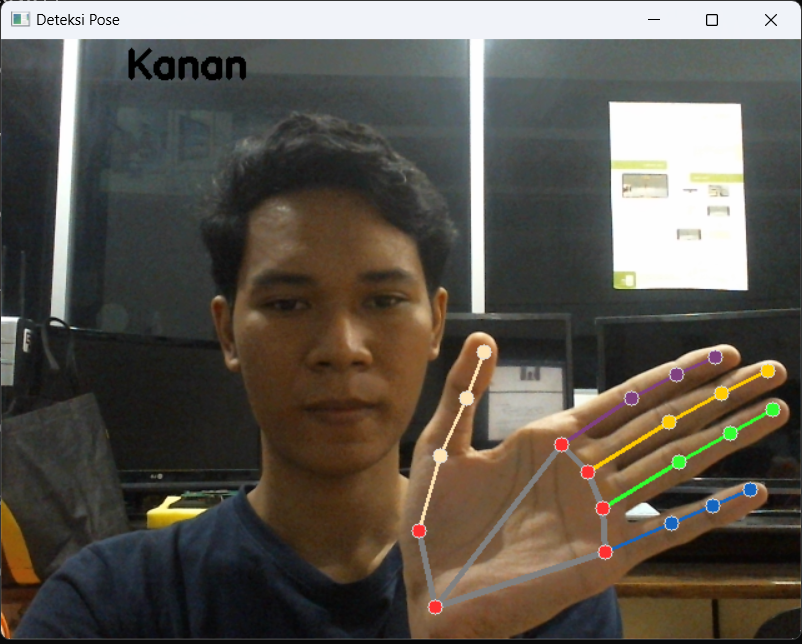
\includegraphics[scale=0.5]{gambar/bab3/Kanan}
  % Keterangan gambar yang diinputkan
  \caption{Contoh citra yang mendeteksi kanan}
  % Label referensi dari gambar yang diinputkan
  \label{fig:klasifikasi kanan}
\end{figure}

\newpage

\subsection{Paket Data}
Untuk dapat menggerakkan kursi roda maka perlu mengirimkan perintah ke kontroler kursi roda. Pada tahap klasifikasi pose telah didapatkan perintah dasar untuk menggerakkan kursi roda, seperti maju, mundur, kanan, kiri, maupun stop. Perintah ini kemudian akan digabungkan dengan kecepatan maksimal menjadi satu \emph{command} atau paket data seperti yang dilihat pada Persamaan \ref{eq:paket-data}.

% Persamaan 3.1
\begin{equation}
  \label{eq:paket-data}
    Arah(char),Kecepatan(integer)
\end{equation}

Variabel arah memiliki tipe data \emph{char} yang akan menentukan gerak dari motor kursi roda, serta variabel kecepatan memiliki tipe data integer yang akan menentukan kecepatan maksimal dari kursi roda. Untuk memperkecil ukuran data maka kode instruksi untuk menentukan arah gerak menggunakan satu huruf untuk mewakili setiap gerakan. Kode instruksi dapat dilihat pada Tabel \ref{tbl:kode-instruksi}. 

% Tabel 3.2
\begin{table}[h]
  \centering
      \caption{Kode instruksi dari hasil klasifikasi}
      \label{tbl:kode-instruksi}
      \begin{tabular}{|c|c|}
          \hline
          Klasifikasi Pose & Kode Instruksi \\ \hline
          Kiri             & A              \\ \hline
          Maju             & B              \\ \hline
          Stop             & C              \\ \hline
          Mundur           & D              \\ \hline
          Kanan            & E              \\ \hline
      \end{tabular}
\end{table}

Setelah kedua variabel tersebut digabungkan maka akan dikirim secara nirkabel, baik menggunakan Bluetooth maupun WiFi dari laptop atau Jetson Nano ke ESP32.

\subsection{Memecahkan Paket Data}
Paket data yang telah dikirimkan melalui laptop maupun Jetson Nano akan diterima oleh ESP32 menggunakan Bluetooth maupun WiFi. Saat diterima oleh ESP32, data tersebut akan menjalani serangkaian proses yang melibatkan pemecahan paket data dan penyesuaian sesuai dengan variabel yang telah ditentukan sebelumnya. Pemecahan paket data ini memungkinkan ESP32 untuk mendekomposisi informasi yang terkandung dalam setiap paket dan memastikan bahwa setiap variabel terpisah dengan akurat. Dengan demikian proses ini akan mengorganisir dan menyusun kembali informasi serta memastikan bahwa setiap variabel telah benar sesuai dengan nama variabel dan tipe data yang disediakan.

\subsection{Kontrol Navigasi}
Kedua variabel yang didapatkan dari pemecahan paket data akan diproses pada ESP32. Variabel arah akan berperan untuk menentukan arah gerak dari motor, sedangkan variabel kecepatan akan digunakan untuk menetapkan kecepatan maksimal dari pergerakan motor tersebut. Terdapat serangkaian logika \emph{if} berantai pada kontrol navigasi, dimana empat variabel dir akan menentukan arah putaran motor. Selain itu, nilai PWM maksimal dikonfigurasi dengan menggunakan variabel kecepatan sehingga pengguna dapat menyesuaikan kecepatan maksimal motor yang pengguna inginkan. Dengan demikian pada tahap ini ESP32 dapat secara efektif memproses data yang diterima melalui sistem nirkabel dan menghasilkan instruksi kontrol yang sesuai untuk menggerakkan kursi roda dengan arah dan kecepatan yang diinginkan.